\documentclass[UTF8]{ctexart}

% 在代码的标题里可以用\protect命令
\usepackage{caption2}

%固定图片位置
\usepackage{float}

%插入超链接
\usepackage{url}

\usepackage{tikz,mathpazo}
\usetikzlibrary{shapes.geometric, arrows}
\usetikzlibrary{calc}

%\usepackage[affil-it]{authblk}

\usepackage{listings}
%插入代码的配置
\definecolor{CPPLight}  {HTML} {686868}
\definecolor{CPPSteel}  {HTML} {888888}
\definecolor{CPPDark}   {HTML} {262626}
\definecolor{CPPBlue}   {HTML} {4172A3}
\definecolor{CPPGreen}  {HTML} {487818}
\definecolor{CPPBrown}  {HTML} {A07040}
\definecolor{CPPRed}    {HTML} {AD4D3A}
\definecolor{CPPViolet} {HTML} {7040A0}
\definecolor{CPPGray}  {HTML} {B8B8B8}
\lstset{
	language=Matlab,                                     % 设置语言
    columns=fixed,    
    breaklines = true,   
    basicstyle=\small ,
    numbers=left,                                        % 在左侧显示行号
    %frame=none,                                          % 不显示背景边框
    backgroundcolor=\color[RGB]{245,245,244},            % 设定背景颜色
    keywordstyle=\color[RGB]{40,40,255}\bfseries,                 % 设定关键字颜色
    %commentstyle=\color{red!10!green!70}\textit,    % 设置代码注释的颜色
    numberstyle=\tiny\color{darkgray},           % 设定行号格式
    commentstyle=\it\color[RGB]{0,96,96},                % 设置代码注释的格式
    stringstyle=\rmfamily\slshape\color[RGB]{128,0,0},   % 设置字符串格式
    showstringspaces=false,                              % 不显示字符串中的空格                           
    %morekeywords={True,alignas,continute,friend,register,true,alignof,decltype,goto,
    %reinterpret_cast,try,asm,defult,if,return,typedef,auto,delete,inline,short,
    %typeid,bool,do,int,signed,typename,break,double,long,sizeof,union,case,
    %dynamic_cast,mutable,static,unsigned,catch,else,namespace,static_assert,using,
    %char,enum,new,static_cast,virtual,char16_t,char32_t,explict,noexcept,struct,
    %void,export,nullptr,switch,volatile,class,extern,operator,template,wchar_t,
    %const,false,private,this,while,constexpr,float,protected,thread_local,
    %const_cast,for,public,throw,std,rand},
    emph={access,and,break,class,continue,def,del,elif ,else,%
	except,exec,finally,for,from,global,if,import,in,i s,%
	lambda,not,or,pass,print,raise,return,try,while, imshow, subplot, figure,%
    log, fft2, fftshift, abs, size, rgb2gray, imread, histeq, imwrite},
    emphstyle=\color{CPPViolet}\bfseries, 
    emph={[2]True, False, None, self},
	emphstyle=[2]\color{green},
	emph={[3]from, import, as},
	emphstyle=[3]\color{blue},
	upquote=true,
	morecomment=[s]{"""}{"""},
    morecomment=[s]{\%}{},
	%commentstyle=\color{orange}\slshape,
    commentstyle=\color{red!10!green!70}\textit,    % 设置代码注释的颜色
	emph={[4]1, 2, 3, 4, 5, 6, 7, 8, 9, 0},
	emphstyle=[4]\color{red},
	emph={[5]numpy, np, plt},
	emphstyle=[5]\color{red},
	literate=*{:}{{\textcolor{blue}:}}{1}%
	{=}{{\textcolor{blue}=}}{1}%
	{-}{{\textcolor{blue}-}}{1}%
	{+}{{\textcolor{blue}+}}{1}%
	{*}{{\textcolor{blue}*}}{1}%
	{!}{{\textcolor{blue}!}}{1}%
	{(}{{\textcolor{blue}(}}{1}%
	{)}{{\textcolor{blue})}}{1}%
	{[}{{\textcolor{blue}[}}{1}%
	{]}{{\textcolor{blue}]}}{1}%
	{<}{{\textcolor{blue}<}}{1}%
	{>}{{\textcolor{blue}>}}{1},%
    %{\%}{{\textcolor{green}\%}}{1},%
	framexleftmargin=0.1mm, framextopmargin=0.1mm, frame=shadowbox, rulesepcolor=\color{black},
}



\usepackage{geometry}
\geometry{left=2cm, right=2cm, top=1.2cm, bottom=1.2cm}

%得到引用的标题内容
\usepackage{nameref} 

%添加首行缩进,两个字符
\usepackage{indentfirst}
\setlength{\parindent}{2em}

%多行公式一个编号
\usepackage{amsmath}

%文献引用,标准类型为plain
%\usepackage[hyperref=true,backend=biber,sorting=none,backref=true]{biblatex}
%\addbibresource{ref.bib}
\bibliographystyle{plain}
\usepackage{cite}

\pagestyle{plain}

%跨页表格
\usepackage{multirow}
\usepackage{longtable,booktabs}
\usepackage{supertabular}
\usepackage{makecell}

%调整itemize等的间距
\usepackage{enumitem}


\usepackage{graphicx}
\usepackage{subfigure}

%超链接
\usepackage[linkcolor=yellow,citecolor=red,backref=page,hyperfootnotes=true]{hyperref}
\hypersetup{
bookmarks=true,
colorlinks=true,
linkcolor=black
}
\usepackage{tabularx} %This package must be placed after package {hyperref}, otherwise footnote marks are NOT treated as hyperlinks.


%引入了一些改进的数学环境,如align
\usepackage{amsmath}

\title{数字图像处理报告七:图像增强}
\author{姓名:鲁国锐 \protect\newline
\and 学号:17020021031 \\
\and 专业:电子信息科学与技术}
\date{2020年4月22日}

\begin{document}
	\maketitle
	\renewcommand{\contentsname}{目录}
	\renewcommand{\listfigurename}{插图目录}
	\renewcommand{\listtablename}{表格目录}
	\renewcommand{\refname}{参考文献}
	\renewcommand{\abstractname}{摘要}
	\renewcommand{\indexname}{索引}
	\renewcommand{\tablename}{表}
	\renewcommand{\figurename}{图}
	
	
	
	\tableofcontents
	\newpage
	
	\hypersetup{
	bookmarks=true,
	colorlinks=true,
	linkcolor=red,
	urlcolor=blue
	}
	\section{题目描述}
                \begin{enumerate}[leftmargin=50pt]
    				\item 在$RGB$和$HSI$空间做图像增强的区别是什么?;
    				\item 如何增强水下图像的色彩?(需要查文献)。
    			\end{enumerate}  

			
%			\begin{figure}[H]
%				\centering 
%				
\includegraphics[scale=0.4]{org_img.png} 
%				\caption{原图及其傅里叶变换} 
%				\label{problem_img}
%			\end{figure}
		


	
	\section{$RGB$空间和$HSI$空间图像增强对比}
        \indent 何为“彩色空间”?教材上给出的解释为\cite{digit_image_Gonzalez}“彩色模型(也称为彩色空间或彩色系统)的目的是,在某些标准下用通常可以接受的方式方便地对彩色加以说明”。其实就是人们对于彩色的一种描述方式。比如本文要讨论的$RGB$模型和$HSI$模型:前者用红、绿、蓝三种原色作为三个分量图像表示一副彩色图像,主要面向硬件;后者则用色调、饱和度、亮度作为分量描述图像,主要面向人类。简单来说,不同的彩色空间的差别就在于所选择的描述标准不同,根据实际的需要,选择最为适合的标准。
        
        \indent 由上述定义我们便可以得到一个对两种方法区别的大体印象:$RGB$空间图像增强方法基于的是对红、绿、蓝三种原色强度的操作;而$HSI$空间基于的是对色调、饱和度、亮度三个指标的操作。下面将进一步对两类方法展开讨论。
        
        
        
        \subsection{$RGB$空间图像增强方法}
            \indent $RGB$空间的图像增强方法主要参考教材\cite{digit_image_Gonzalez}第$3$章中的方法,大体可以分为以下几类:
            
                \begin{enumerate}[leftmargin=50pt]
                    \item 基于灰度变换函数的方法:通过将整幅图像的像素经过一个或多个函数映射达到增强的目的,典型的方法有对比度拉伸变换和伽马变换等;
    				\item 基于直方图处理的方法:通过对三个通道中像素的统计特性进行操作来达到增强的目的,典型的方法有直方图均衡和直方图匹配等;
    				\item 基于锐化空间滤波器的方法:通过对像素的直接操作(主要是微分或差分)来提取图像的边缘特性,将其加到原图像上以达到增强的目的,典型的方法有拉普拉斯算子和$Sobel$算子等。
    			\end{enumerate}              
                
           \indent 上述方法最大的缺点是:由于三个通道的像素值分布往往不一样,所以在进行处理后会导致图像各分量的比例发生变化,使得颜色偏离了实际的样子。
           
           \indent 注意这里并未将第$4$章中的频率域滤波方法加入进来,因为个人认为当将一副图像变换到频率域之后,对图像的描述方式也相应地变了(由红、绿、蓝三原色变为了三个通道的频率的相位和幅度),超出了$RGB$彩色空间的表示范围。
           
           \subsubsection{实验思路}
                \indent 分别对$R$、$G$、$B$三个通道进行直方图均衡,观察实验结果,尤其是色调是否产生变化。
           
           \subsubsection{实验代码}

       \begin{lstlisting}[language=Matlab,caption={分别对三个通道进行直方图均衡操作}]
%函数histeq()进行直方图均衡化处理
I=imread('3153987-fd1e1de03f59e3a8.jpeg');
J=histeq(I);  %直方图均衡化

J(:, :, 1) = histeq( I(:, :, 1) );
J(:, :, 2) = histeq( I(:, :, 2) );
J(:, :, 3) = histeq( I(:, :, 3) );
% J = histeq(I);

figure,
subplot(221),imshow(I);
title('原图')
subplot(222),imshow(J);
title('均衡化后')
subplot(223),imhist(I,64);
title('原图像直方图');
subplot(224),imhist(J,64);
title('均衡化后的直方图');

imwrite(J, 'C:\Users\Asus-\Desktop\数字图像\codes\contrast_stretching\test.png');

       \end{lstlisting}
       
       \subsubsection{实验结果}
                                   \begin{figure}[H]
                                       \centering
                                       \subfigure[原图]{
                                           \begin{minipage}{0.45\linewidth}
                                               \centering
                                               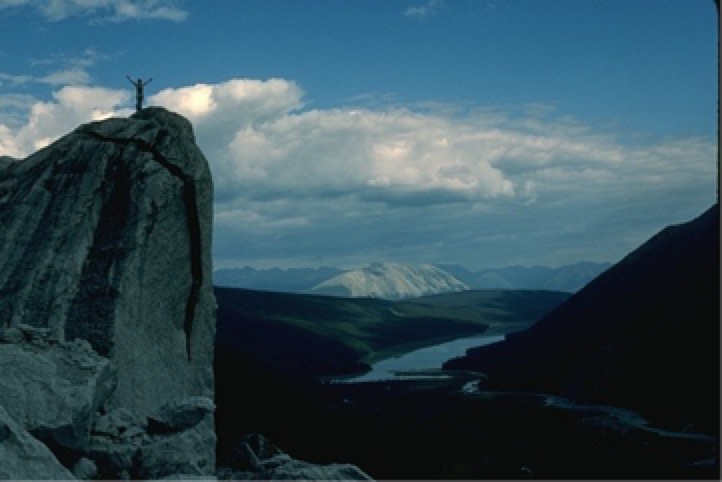
\includegraphics[scale=0.32]{3153987-fd1e1de03f59e3a8.jpeg}
                                               %\caption{原图3}
                                               \label{hist_orig}
                                           \end{minipage}
                                       }
                                       \subfigure[经直方图均衡处理后的结果]{
                                           \begin{minipage}{0.45\linewidth}
                                               \centering
                                               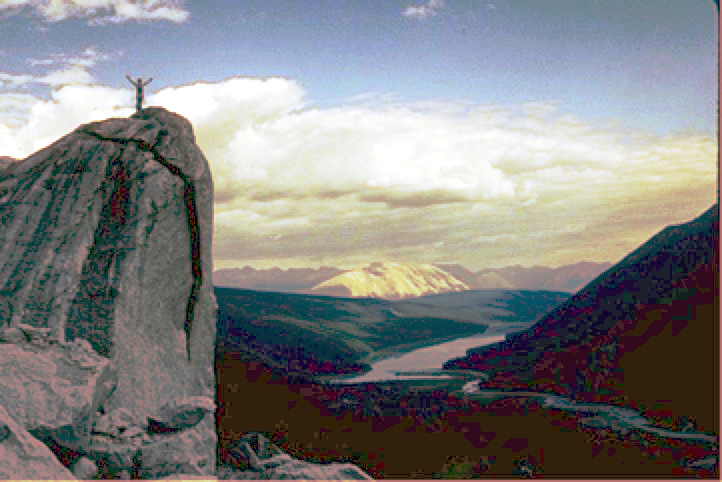
\includegraphics[scale=0.32]{test.png}
                                               %\caption{结果3}
                                               \label{hist_res}
                                           \end{minipage}
                                       }
                                       
                                       \caption{对图像进行直方图均衡操作后可能会导致颜色偏离原始色彩\protect\footnotemark[1]}
                                       \label{butterworth}
                                   \end{figure}
            
            \indent 如图\ref{hist_orig}和图\ref{hist_res}所示,分别对$R$、$G$、$B$三个通道进行直方图均衡后的结果,其部分区域的色调发生了明显改变,如云的颜色,有偏蓝变成了金黄。
            
            \indent 另外需要注意的一点是,\textbf{并不是对所有的图像进行上述操作都会导致色调的改变},此次实验中尝试了若干幅图像,目前只有图\ref{hist_orig}这一张能非常明显地看到色调被改变了。
            
            \footnotetext[1]{原图来源于网络:\url{https://www.jianshu.com/p/5a8d12d6c649}}
        
        \subsection{$HSI$空间图像增强方法}
        
            \indent 在$HSI$彩色空间中进行图像增强最大的好处是\cite{song2017基于HSI}:“各颜色分量是相互独立的,这样就可以消除各颜色分量之间的相关性,所以保持色调分量($hue,H$)不变,只需调整饱和度分量($saturability,S$)和亮度分量($intensity,I$)就可达到增强图像的目的。”
            
            \indent 从上面的话可以得出,在$HSI$空间对图像进行增强,只要不去改动$H$分量,理论上就不会对结果的色调产生影响。
            \subsubsection{实验思路}
                \indent 将一副$RGB$图像变换到$HSI$空间,只对其强度分量进行直方图均衡,再变换回$RGB$空间,观察实验结果。
            
            \subsubsection{实验代码}
\begin{lstlisting}[language=Matlab,caption={在$HST$彩色空间对强度分量做直方图均衡\protect\footnotemark[1]}]
% 读取图像显示原图
img = imread('3153987-fd1e1de03f59e3a8.jpeg');
figure(1)
imshow(img)
title('原图')

img_hsi = rgb2hsi(img);% 转到HSI空间
img_hsi(:, :, 3) = histeq( img_hsi(:, :, 3) );% 对强度进行直方图均衡
img = hsi2rgb(img_hsi);
figure(3)
imshow(img)
title('对强度进行直方图均衡后的结果')
imwrite(img, 'C:\Users\Asus-\Desktop\数字图像\report\07\enhanced_res_using_hsi.png')
       \end{lstlisting}   
       
       \footnotetext{$MATLAB$没有现成的$RGB$与$HSI$空间相互转换的函数,代码中$rgb2hsi$和$hsi2rgb$这两个函数取自本课程实验五提供的资料,即冈萨雷斯所著的《数字图像处理(MATLAB)版》中提供的的代码。}
            \subsubsection{实验结果}  
            
                   
                                   \begin{figure}[H]
                                       \centering
                                       \subfigure[原图]{
                                           \begin{minipage}{0.45\linewidth}
                                               \centering
                                               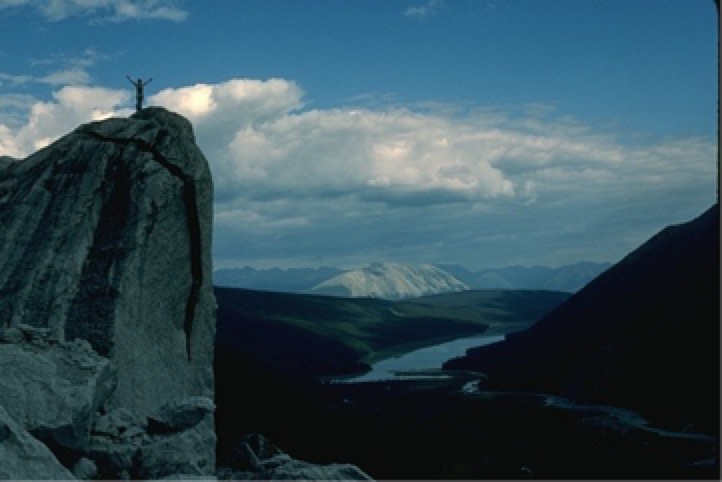
\includegraphics[scale=0.32]{3153987-fd1e1de03f59e3a8.jpeg}
                                               %\caption{原图3}
                                               \label{hist_orig_hsi}
                                           \end{minipage}
                                       }
                                       \subfigure[只针对强度分量进行直方图均衡后的结果]{
                                           \begin{minipage}{0.45\linewidth}
                                               \centering
                                               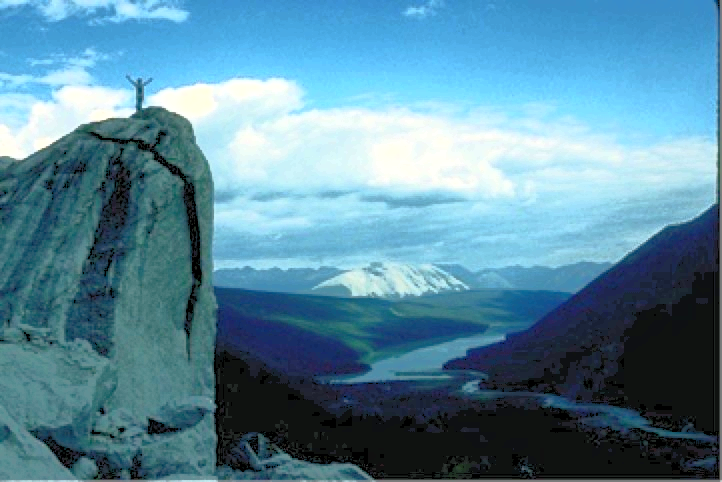
\includegraphics[scale=0.32]{enhanced_res_using_hsi.png}
                                               %\caption{结果3}
                                               \label{hist_res_hsi}
                                           \end{minipage}
                                       }
                                       
                                       \caption{在$HSI$空间对强度分量进行直方图均衡可以有效缓解色调改变的问题}
                                       \label{butterworth}
                                   \end{figure}
                                   
                \indent 如图\ref{hist_orig_hsi}和图\ref{hist_res_hsi}所示,在$HSI$空间对强度分量进行直方图均衡后,其结果对比度有明显提高,同时色调也能与原图保持一致。                       
                                       
    \section{水下图像增强}
    
        \subsection{概述}
            \indent 海洋中拥有着丰富的资源,具有巨大的开发潜力。水下光学图像作为传输海洋信息的主要载体,对探索与开发海洋起着至关重要的作用\cite{lin2020基于优势特征图像融合的水下光学图像增强}。然而,由于海水的良导体特性,再加之水体中微粒杂志的散射作用,导致光在水中传播时会有强烈的衰减,使得水下图像往往会出现失真、模糊、对比度低等问题\cite{zou2020非均匀光照}。因此,如何有效地提升水下光学图像的质量是一个亟待解决的问题。
            
            \indent 在\cite{lin2020水下图像处理技术}中,作者总结了水下图像增强的五类主要方法,分别为:

                \begin{enumerate}[leftmargin=50pt]
                    \item 基于直方图的水下图像增强算法;
                    \item 基于$Retinex$的水下图像增强算法;
                    \item 基于滤波和信号处理的水下图像增强算法;
                    \item 基于图像融合的水下图像增强算法;
                    \item 基于$CNN$的水下图像增强算法。
    			\end{enumerate}                 
            
            \indent 另外,在多篇关于水下图像增强的文献中\cite{lin2020水下图像处理技术}\cite{lin2020基于优势特征图像融合的水下光学图像增强}\cite{zou2020非均匀光照},都引用了同一个算法——由何恺明等人提出的暗通道先验算法\cite{he2010single}。可见该算法对于水下图像增强有着重要意义,本次报告将在接下来的一节中着重介绍这一算法。
            
        \subsection{暗通道先验算法}
            \subsubsection{原理:暗通道先验}\label{principle : dark channel prior}
                \indent 论文提出的算法基于一个非常简单事实:在一张没有雾的图像中,除了类似于天空这样的区域,其余地方像素的$R$、$G$、$B$三个通道一般会有至少一个通道的强度非常小。为了说明这样一个事实,作者提出了“暗通道”这一概念,它的定义由公式\ref{definition : dark channel}给出:
                
                    \begin{align}
                        J^{dark} \left( \mathbf{x} \right) = \mathop{min}\limits_{ y \in \Omega \left( \mathbf{x} \right)} \left( \mathop{min}\limits_{c \in \left\{ r, g, b \right\}  }  J^c \left( \mathbf{y} \right)    \right)  \label{definition : dark channel}
                    \end{align}
                    
                \indent 公式\ref{definition : dark channel}的意思是对图像中的每一个像素,取出它$R$、$G$、$B$三个通道中的最小值,得到一个与原图长宽一样的二维矩阵,再对这个二维矩阵进行一次最小值滤波,得到的即为暗通道。论文里对为何还要在进行一次最小值滤波的原因没有详细说明,个人猜测应当是\textbf{为了消除部分类似于天空这样的区域的干扰},因为天空区域往往没有暗通道,其三个分量的强度都比较大。
                
                \indent 用暗通道来表示论文提出的事实,可以写成:对于一张没有雾的自然图像,有:
                    \begin{align}
                        J^{dark} \rightarrow 0 \label{dark channel : tend to be 0}
                    \end{align}
                    
                \indent 作者将这个称为“暗通道先验”。
                
                \indent 为了证明这一事实的普遍性,作者还随机选取了$5000$张图片,裁剪掉天空区域,统计了剩余部分暗通道中的像素值(如图\ref{statistic}所示),结果显示,大约有$85\%$的像素值在$16$以下,大约$75\%$的像素值为$0$。
    			
    			\begin{figure}[htbp]
    				\centering 
         			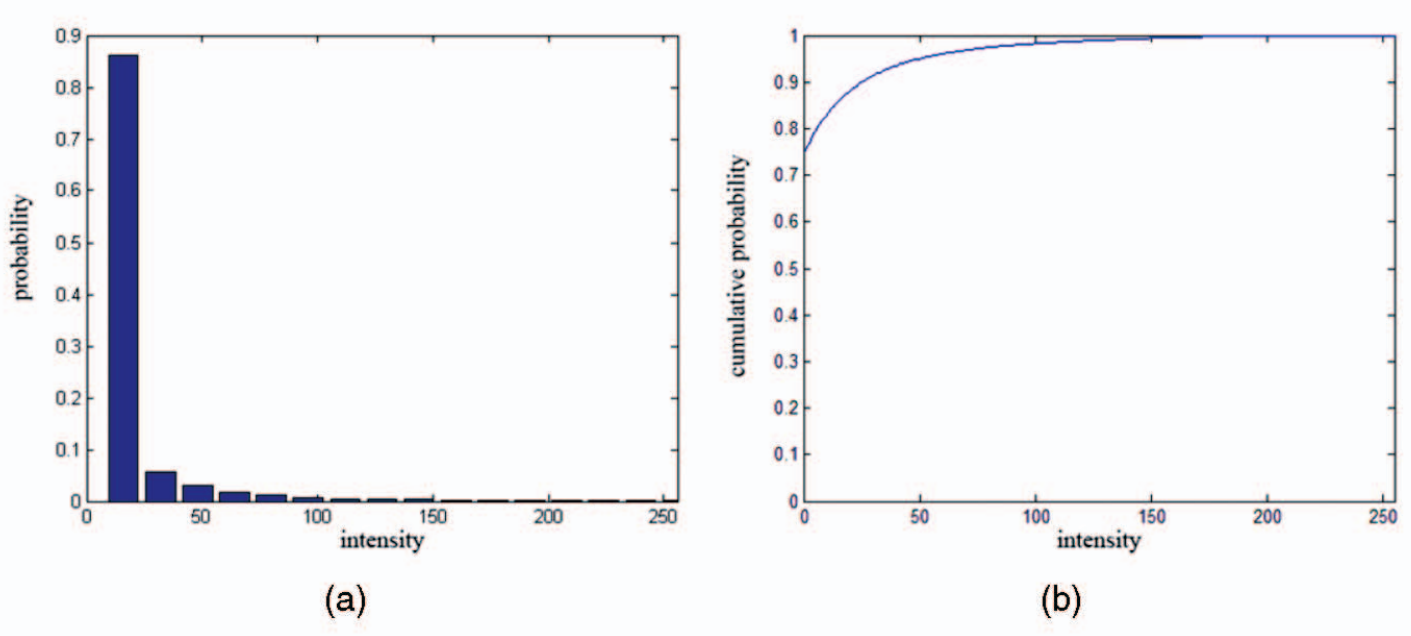
\includegraphics[scale=0.5]{statistic.png} 
    				\caption{暗通道像素值统计结果} 
    				\label{statistic}
    			\end{figure}
        
            \subsubsection{原理:模型} \label{principle : model}
            
            \indent 在计算机视觉和计算机图形学中,雾图像可以被建模为:  
                \begin{align}
                    \mathbf{I}\left( \mathbf{x} \right) = \mathbf{J}\left( \mathbf{x} \right) t\left( \mathbf{x} \right) + \mathbf{A}\left( 1 - t\left( \mathbf{x} \right) \right) \label{model : haze image}
                \end{align}
                     
            \indent 其中$\mathbf{I}$是待去雾的图像;$\mathbf{J}$是无雾的图像;$t\left( x \right)$是媒质传播函数,用以描述没有被散射的、到达相机上的光的比例;$\mathbf{A}$是全局大气光照。去雾的任务就是要求出$t\left( x \right)$和$\mathbf{A}$以解出$\mathbf{J}$。
            
            \subsubsection*{大气光照$\mathbf{A}$的求解}
                \indent 在过去的工作中,一般用雾图像中最不透明区域的颜色来表示$\mathbf{A}$。当太阳光可以被忽略时,大气光就是图像中唯一的光源。此时有:
                    \begin{align}
                        J\left( \mathbf{x} \right) = R\left( \mathbf{x} \right)A \label{model : no haze when sunlight ignored}
                    \end{align}
                
                \indent 将\ref{model : no haze when sunlight ignored}式代入\ref{model : haze image}式,可得:
                    \begin{align}
                        I\left( \mathbf{x} \right) = R\left( \mathbf{x} \right)At\left( \mathbf{x} \right) + \left( 1 - t\left( x \right) \right)A \label{model : haze when sunlight ignored}
                    \end{align}
                    
                \indent 又因为
                    \begin{align}
                        t\left( \mathbf{x} \right) = e^{-\beta d\left( \mathbf{x} \right)} \label{model : definition of t}
                    \end{align}
                    
                \indent 这里$\beta$表示大气光的散射系数,$d$表示景深。所以当景深趋近于无穷大的点存在于图像中时,$\mathop{lim}\limits_{d \to \infty}t\left( \mathbf{x} \right)$趋于$0$。代入\ref{model : haze when sunlight ignored}式,可得:
                    \begin{align}
                        \lim_{d \to +\infty}I\left( \mathbf{x} \right) &= R\left( \mathbf{x} \right)A\lim_{d \to +\infty}t\left( \mathbf{x} \right) + \left( 1 - \lim_{d \to +\infty}t\left( x \right) \right)A \\
                        &= A
                    \end{align}
                
                \indent 作者从这里直接得出了此时图中最亮的点就是雾图像中最不透明区域的颜色,并且它的值近似等于$A$。也就是说,$\mathop{lim}\limits_{d \to \infty}I\left( \mathbf{x} \right)$所表示的就是图中最亮的点。这一结论对我而言似乎并不是显而易见的,暂时还没有想明白为什么。
                
                \indent 接下来,文中又提到,太阳光往往是不能忽略的,所以\ref{model : no haze when sunlight ignored}式需要被修正为:
                    \begin{align}
                        J\left( \mathbf{x} \right) = R\left( \mathbf{x} \right)\left( A + S\right) \label{model : no haze when sunlight considered}
                    \end{align}
                    
               \indent 代入\ref{model : haze image}式得:
                    \begin{align}
                        I\left( \mathbf{x} \right) = R\left( \mathbf{x} \right)St\left( \mathbf{x} \right) + R\left( \mathbf{x} \right)At\left( \mathbf{x} \right) + \left( 1 - t\left( x \right) \right)A \label{model : haze when sunlight considered}
                    \end{align}
                    
                \indent 作者认为此时图像中最亮的点比大气光更亮,不能直接用来求$A$。同样,这里关于$\mathop{lim}\limits_{d \to \infty}I\left( \mathbf{x} \right)$和最亮的点之间的关系我并没有想明白,也暂时略过。
                
                \indent 于是作者提出可以用暗通道来估计大气光。算法如下:
                
                    \begin{enumerate}[leftmargin=50pt]
                        \item 对暗通道中的点按强度降序排序,选取前$0.1\%$的点;
                        \item 获取这些点在暗通道中的坐标,也就是不透明区域在原图中的坐标;
                        \item 在原图中遍历这些坐标,找出最亮的点,即得$A$。
        			\end{enumerate}  
                
                \indent 按照作者所说的,暗通道中强度排在前$0.1\%$的点往往表示的就是是雾图像中最不透明的区域,按大气光的定义,只需在这样的区域中找到最亮的点就得到$A$了。
                
                \indent 至于为什么暗通道中强度排在前$0.1\%$的点能够表示雾图像中最不透明的区域,个人猜测是因为\textbf{对暗通道做了最小值滤波,将太阳光的影响给滤除了}。正如\ref{principle : dark channel prior}中所猜测的那样,最小值滤波是为了消除类似于天空这样的区域的干扰。现在看来,\textbf{所谓“天空这样的区域的干扰”应该指的就是太阳光的干扰}。
                
            \subsubsection*{媒质传递函数$t\left( \mathbf{x} \right)$的求解}
                \indent 对\ref{model : haze image}式两边同时除以$A$,得:
                    \begin{align}
                        \frac{ I^{c}\left( \mathbf{x} \right) }{ A^c } = t\left( \mathbf{x} \right)\frac{J^{c}\left( \mathbf{x} \right)}{A^c} + 1 - t\left( \mathbf{x} \right) \label{model : haze image by A}
                    \end{align}
                    
                \indent 对\ref{model : haze image by A}两边同时求暗通道,得:
                    \begin{align}
                        \mathop{min}\limits_{ y \in \Omega \left( \mathbf{x} \right)} \left( \mathop{min}\limits_{c \in \left\{ r, g, b \right\}  }  \frac{ I^c \left( \mathbf{y} \right) }{A^c} \right) = \widetilde{t}\left( \mathbf{x} \right) \mathop{min}\limits_{ y \in \Omega \left( \mathbf{x} \right)} \left( \mathop{min}\limits_{c \in \left\{ r, g, b \right\}  }  \frac{ J^c \left( \mathbf{y} \right)}{ A^c } \right) + 1 - \widetilde{t}\left( \mathbf{x} \right) \label{model : dark channel of haze image}
                    \end{align}
                    
                \indent 由于$\widetilde{t}\left( \mathbf{x} \right)$在滤波时是一个常数(为什么?),所以可以提到算子的外面。再根据暗通道先验理论,将\ref{definition : dark channel}式代入\ref{model : dark channel of haze image}式,可得:
                    \begin{align}
                        \widetilde{t}\left( \mathbf{x} \right) = 1 -  \mathop{min}\limits_{ y \in \Omega \left( \mathbf{x} \right)} \left( \mathop{min}\limits_{c \in \left\{ r, g, b \right\}  }  \frac{ I^c \left( \mathbf{y} \right) }{A^c} \right) \label{model : solution of t}
                    \end{align}
                    
                \indent 作者提到,对于雾图像中的天空区域颜色很趋近于大气光$A$,所以在天空区域有:
                    \begin{align}
                        \mathop{min}\limits_{ y \in \Omega \left( \mathbf{x} \right)} \left( \mathop{min}\limits_{c \in \left\{ r, g, b \right\}  }  \frac{ I^c \left( \mathbf{y} \right) }{A^c} \right) \rightarrow 1 \label{model : sky region}
                    \end{align}
                    
                \indent 所以\ref{model : solution of t}式在天空区域求出来的值会趋于$0$,所以不需要单独考虑天空,\ref{model : solution of t}可以同时处理天空和非天空区域。然而,我并没有看出天空区域的$t$趋于$0$和该公式可以直接处理天空区域之间的逻辑关系。实际上,\textbf{从最后求解$J$的公式(下一节给出)来看,$t$趋于$0$反而会加剧对该区域的作用,因为$t$出现在分母上}。
                
                \indent 作者还提到,即便是晴朗的天气下,也是有雾存在的;而且,雾还是人感知深度的一条线索。所以如果把雾彻底去除,图像看起来反而会不自然。因此还需用一个参数$\omega$对\ref{model : solution of t}式进行修正:
                    \begin{align}
                        \widetilde{t}\left( \mathbf{x} \right) = 1 -  \omega \mathop{min}\limits_{ y \in \Omega \left( \mathbf{x} \right)} \left( \mathop{min}\limits_{c \in \left\{ r, g, b \right\}  }  \frac{ I^c \left( \mathbf{y} \right) }{A^c} \right) \label{model : final solution of t}
                    \end{align}
                    
                \indent 这里$\omega$介于$0$到$1$之间,论文里的所有结果都是取的$0.95$。
                
            \subsubsection*{无雾图像$J$的求解}
                \indent 至此,所有的位置参数都已求出,解\ref{model : haze image}式,可得:
                    \begin{align}
                        \mathbf{J}\left( \mathbf{x} \right) = \frac{ \mathbf{I}\left( \mathbf{x} \right) - \mathbf{A} }{ t\left( \mathbf{x} \right) } + \mathbf{A} \label{model : solution of J}
                    \end{align}
                    
                \indent 当$t\left( \mathbf{x} \right)$很小的时候,可能会导致结果出现噪声,需要对$t\left( \mathbf{x} \right)$进行限制,对\ref{model : solution of J}式进行修正,得到最终的表达式为:
                    \begin{align}
                        \mathbf{J}\left( \mathbf{x} \right) = \frac{ \mathbf{I}\left( \mathbf{x} \right) - \mathbf{A} }{ \mathop{max}\left( t\left( \mathbf{x} \right), t_0 \right) } + \mathbf{A} \label{model : final solution of J}
                    \end{align}
                    
                \indent 式中$t_0$的标准值为$0.1$。
        
            \subsubsection{算法复现}
\begin{lstlisting}[language=Matlab,caption={暗通道先验算法代码复现\protect\footnotemark[1]}]
classdef dark_channel_prior < handle
   
    properties( SetAccess=private, GetAccess=public )
        % 在构造函数中初始化的变量
        im_path;% 图像路径
        I;% 读取的图像,待去雾
        M;% 图像的行数
        N;% 图像的列数
        path;% 读取的图像所在路径
        name;% 所读图像文件名
        ext;% 所读图像的扩展名
        
        % 待求变量
        dark_channel;% 图像的暗通道
        dark_path;% 暗通道结果路径
        tx;% the medium transmission,媒介传播函数 
        A;% global atmospheric light,大气光
        I_by_A;% I^c / A^c
        I_by_A_dark;% I^c / A^c的暗通道
        %A_loc;% A在I中的位置
        J;% 去雾后的图像
        num;% 前num个最大值,用于求A
        
        % 常数,有默认值
        w;% 一个常系数,用于保留一定的雾,默认0.95
        patch_size;% 最小值滤波的滤波器大小,默认15X15
        t0;% 防止t太小导致结果有噪声,默认0.1
        
    end
    
    methods
        % 构造函数
        function obj = dark_channel_prior(im_path, varargin)
            
            % 设置默认参数
            obj.w = 0.95;
            obj.patch_size = 15;
            obj.t0 = 0.1;
            if length(varargin) == 1
                obj.w = varargin{1};
            elseif length(varargin) == 2
                obj.w = varargin{1};
                obj.patch_size = varargin{2};
            elseif length(varargin) == 3
                obj.w = varargin{1};
                obj.patch_size = varargin{2};
                obj.t0 = varargin{3};
            end
                
            
            % 初始化成员变量
            obj.im_path = im_path;
            obj.I = imread(im_path);
            obj.I = im2double(obj.I);
            [obj.M, obj.N, ~] = size(obj.I);
            [obj.path, obj.name, obj.ext] = fileparts(im_path);
            obj.path = strcat(obj.path, '\');
            obj.num = round( obj.M * obj.N / 1000 );
            
            % 执行去雾操作
            obj.dehaze();
        end
        
        
    end
    
    methods 
        % 求暗通道
        function img_dark = find_dark_channel(obj, img)
            % 取每个通道上的最小值 
            img_dark = min( img, [], 3 );
            % 最小值滤波
            img_dark = ordfilt2( img_dark, 1, ones(obj.patch_size), 'symmetric');
        end
    end
        
    methods
        % 求A
        function find_A(obj)
            t = sort( obj.dark_channel(:), 'descend' );
            [m, n] = find( obj.dark_channel >= t(obj.num), obj.num);
            obj.A = [0, 0, 0];
            %obj.A_loc = [0, 0];
            for x = 1 : obj.num
%                 intensity = max( obj.I( m(x), n(x), : ) );
%                 if intensity > max(obj.A)
%                     obj.A(1) = obj.I( m(x), n(x), 1 );
%                     obj.A(2) = obj.I( m(x), n(x), 2 );
%                     obj.A(3) = obj.I( m(x), n(x), 3 );
%                 end
                if obj.I( m(x), n(x), 1) > obj.A(1)
                    obj.A(1) = obj.I( m(x), n(x), 1);
                end
                if obj.I( m(x), n(x), 2) > obj.A(2)
                    obj.A(2) = obj.I( m(x), n(x), 2);
                end
                if obj.I( m(x), n(x), 3) > obj.A(3)
                    obj.A(3) = obj.I( m(x), n(x), 3);
                end

            end
            
        end
    end
    
    
    methods
        % 求tx
        function find_tx(obj)
            obj.tx = zeros( obj.M, obj.N );
            obj.I_by_A = obj.I;
            obj.I_by_A(:, :, 1) = obj.I_by_A(:, :, 1) / obj.A(1);
            obj.I_by_A(:, :, 2) = obj.I_by_A(:, :, 2) / obj.A(2);
            obj.I_by_A(:, :, 3) = obj.I_by_A(:, :, 3) / obj.A(3);
            obj.I_by_A_dark = obj.find_dark_channel( obj.I_by_A );
            obj.tx = 1 - obj.w * obj.I_by_A_dark;
        end
    end
    
    methods
        % 去雾
        function dehaze(obj)
            % 求原图像的暗通道并显示
            obj.dark_channel = obj.find_dark_channel( obj.I );
            figure
            imshow(obj.dark_channel);
            title('暗通道')
            obj.dark_path = strcat( obj.path, obj.name );
            obj.dark_path = strcat( obj.dark_path, '_dark.png');
            imwrite( obj.dark_channel, obj.dark_path );
            
            % 求A,结果存放在obj.A中
            obj.find_A();
            %求tx,结果存放在obj.tx中
            obj.find_tx();
            
            obj.J = obj.I;
            for x = 1 : obj.M
                for y = 1 : obj.N
                    for c = 1 : 3
                        obj.J(x, y, c) = obj.I(x, y, c) - obj.A(c);
                        obj.J(x, y, c) = obj.J(x, y, c) / max( obj.tx(x, y), obj.t0);
                        obj.J(x, y, c) = obj.J(x, y, c) + obj.A(c);
                    end
                end
            end
            
            figure
            imshow(obj.J)
            title('去雾后的结果')
            res_path = strcat( obj.path, obj.name);
            res_path = strcat( res_path, 'res.jpg');
            imwrite( obj.J, res_path );

        end
    end
end
       \end{lstlisting}
            
            
            \subsubsection{实验结果}

                                   \begin{figure}[H]
                                       \centering
                                       \subfigure[原图1]{
                                           \begin{minipage}{0.45\linewidth}
                                               \centering
                                               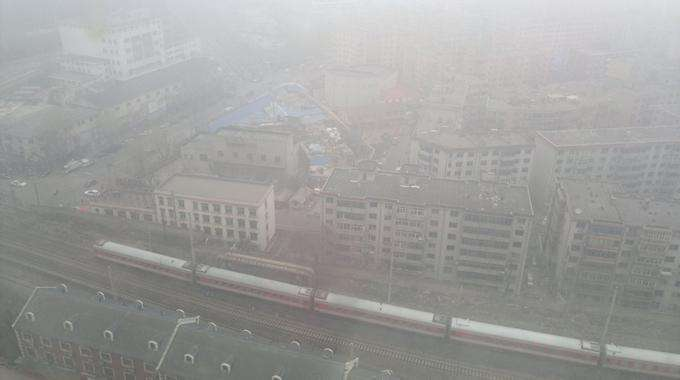
\includegraphics[scale=0.34]{./haze/01.jpg}
                                               %\caption{原图3}
                                               \label{dehaze_orig00}
                                           \end{minipage}
                                       }
                                       \subfigure[去雾结果1]{
                                           \begin{minipage}{0.45\linewidth}
                                               \centering
                                               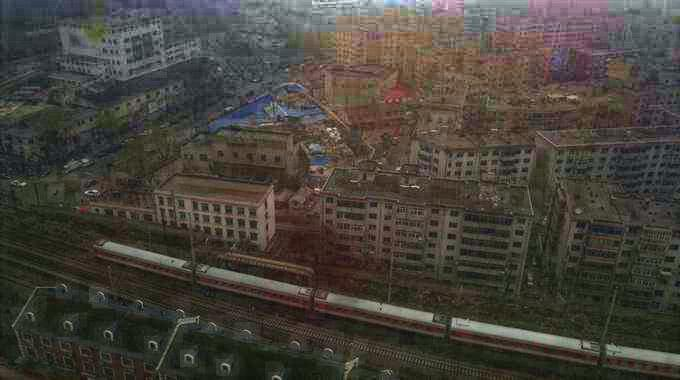
\includegraphics[scale=0.34]{./haze/01res.jpg}
                                               %\caption{结果3}
                                               \label{dehaze_res00}
                                           \end{minipage}
                                       }
                                       
                                       \caption{结果1}
                                       \label{dehaze00}
                                   \end{figure} 

                                   \begin{figure}[H]
                                       \centering
                                       \subfigure[原图2]{
                                           \begin{minipage}{0.45\linewidth}
                                               \centering
                                               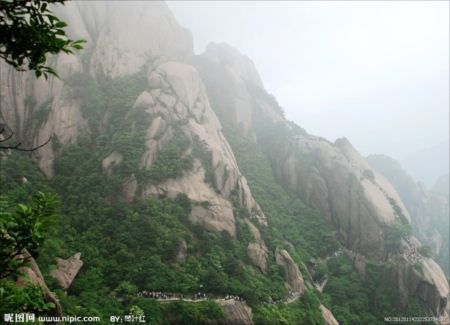
\includegraphics[scale=0.51]{./haze/02.jpg}
                                               %\caption{原图3}
                                               \label{dehaze_orig02}
                                           \end{minipage}
                                       }
                                       \subfigure[去雾结果2]{
                                           \begin{minipage}{0.45\linewidth}
                                               \centering
                                               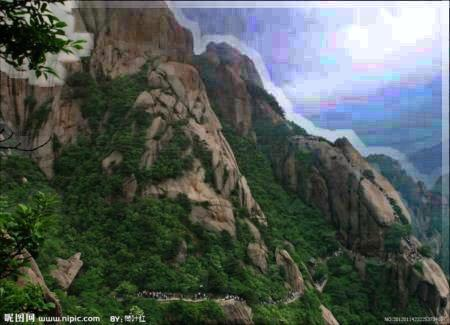
\includegraphics[scale=0.51]{./haze/02res.jpg}
                                               %\caption{结果3}
                                               \label{dehaze_res02}
                                           \end{minipage}
                                       }
                                       
                                       \caption{结果2}
                                       \label{dehaze02}
                                   \end{figure} 
                                   
                                   \begin{figure}[H]
                                       \centering
                                       \subfigure[原图3]{
                                           \begin{minipage}{0.45\linewidth}
                                               \centering
                                               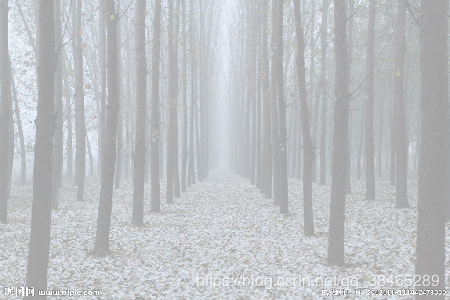
\includegraphics[scale=0.51]{./haze/03.png}
                                               %\caption{原图3}
                                               \label{dehaze_orig03}
                                           \end{minipage}
                                       }
                                       \subfigure[去雾结果3]{
                                           \begin{minipage}{0.45\linewidth}
                                               \centering
                                               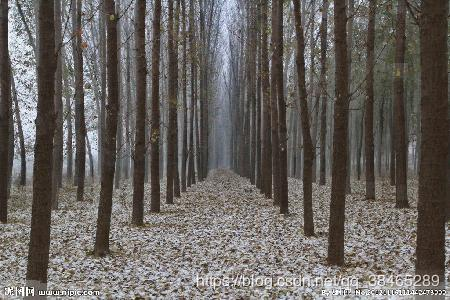
\includegraphics[scale=0.51]{./haze/03res.jpg}
                                               %\caption{结果3}
                                               \label{dehaze_res03}
                                           \end{minipage}
                                       }
                                       
                                       \caption{结果3}
                                       \label{dehaze03}
                                   \end{figure}                                                   

                                   \begin{figure}[H]
                                       \centering
                                       \subfigure[原图4]{
                                           \begin{minipage}{0.45\linewidth}
                                               \centering
                                               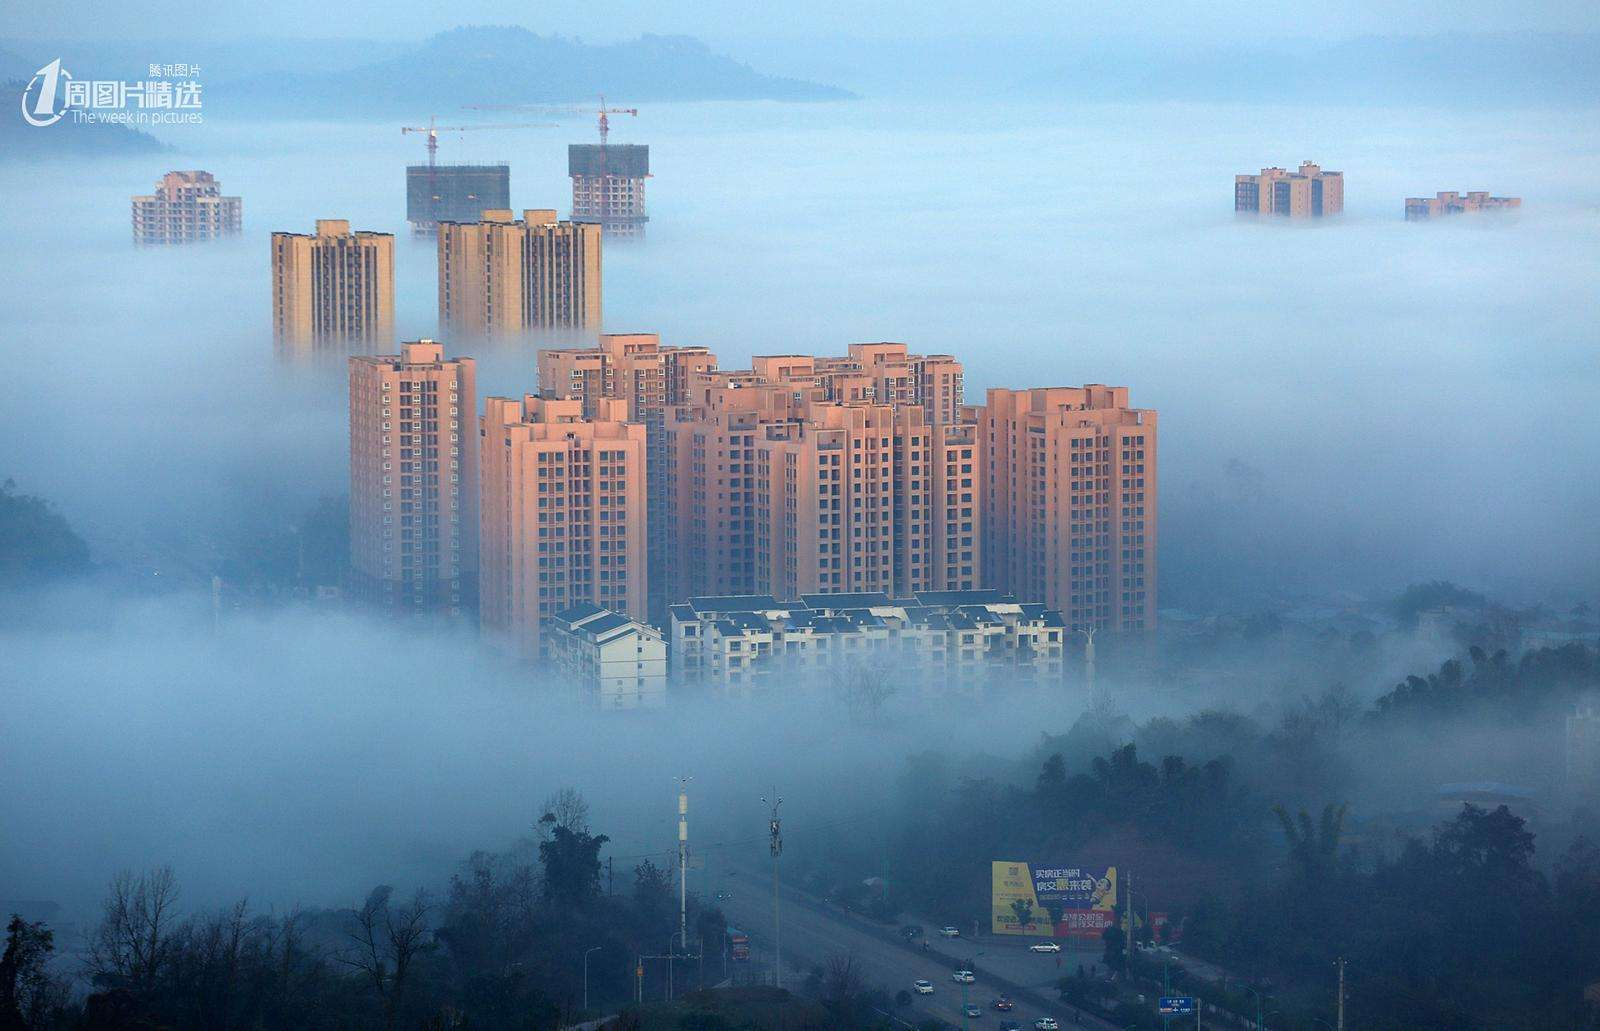
\includegraphics[scale=0.144]{./haze/04.jpg}
                                               %\caption{原图3}
                                               \label{dehaze_orig04}
                                           \end{minipage}
                                       }
                                       \subfigure[去雾结果4]{
                                           \begin{minipage}{0.45\linewidth}
                                               \centering
                                               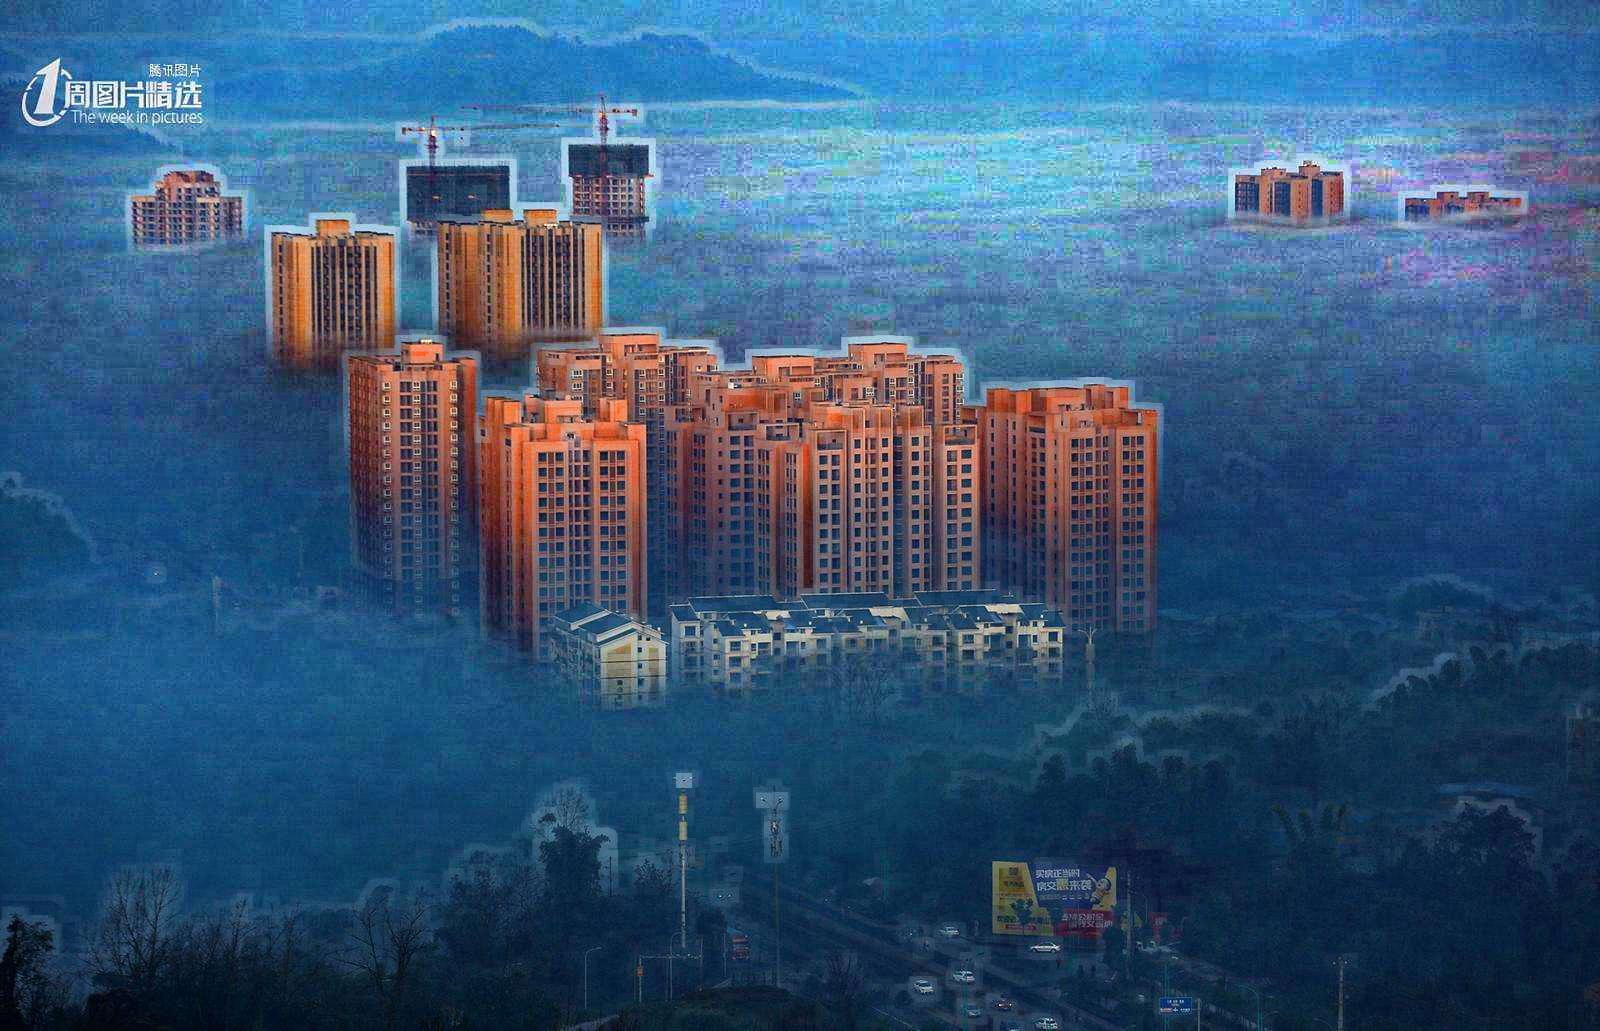
\includegraphics[scale=0.144]{./haze/04res.jpg}
                                               %\caption{结果3}
                                               \label{dehaze_res04}
                                           \end{minipage}
                                       }
                                       
                                       \caption{结果4}
                                       \label{dehaze04}
                                   \end{figure} 
                                   
                                   \begin{figure}[H]
                                       \centering
                                       \subfigure[原图5]{
                                           \begin{minipage}{0.45\linewidth}
                                               \centering
                                               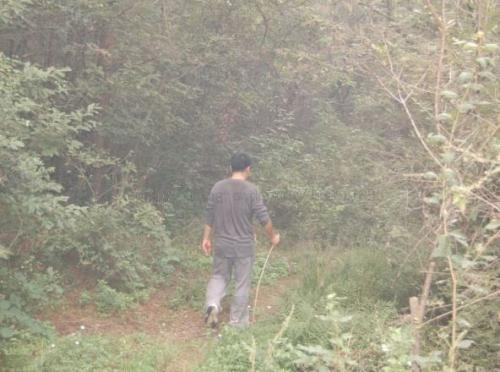
\includegraphics[scale=0.46]{./haze/09.jpg}
                                               %\caption{原图3}
                                               \label{dehaze_orig05}
                                           \end{minipage}
                                       }
                                       \subfigure[去雾结果5]{
                                           \begin{minipage}{0.45\linewidth}
                                               \centering
                                               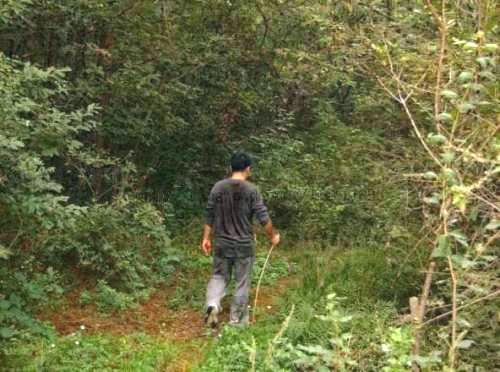
\includegraphics[scale=0.46]{./haze/09res.jpg}
                                               %\caption{结果3}
                                               \label{dehaze_res05}
                                           \end{minipage}
                                       }
                                       
                                       \caption{结果5}
                                       \label{dehaze05}
                                   \end{figure}                                   
                \indent 其实论文中还有一个环节$Soft\ Matting$,由于这一节实在是没看懂,所以最终没有实现这一块。得到的结果质量也不如论文中的稳定。图\ref{dehaze02}图\ref{dehaze05}所示的结果还比较不错,在去除了雾的同时还大体能维持色调不变。但剩余的三幅图像颜色失真就比较严重,尤其是天空所在的区域。正如本次报告在\ref{principle : model}中提出的那样,\textbf{\ref{model : definition of t}式究竟能否处理天空区域?为什么?}
                
                \indent 另外,从图\ref{dehaze02}和图\ref{dehaze04}中可以看到,去雾后的图像边界有明显的白带。对比论文中的$Fig.\ 6$,可以知道这些白带产生原因是由于未加$Soft\ Matting$而造成的。
            
%        \nocite{digit_image_Gonzalez}
%        \nocite{signal_and_system}
%        \nocite{discrete-time_signal_processing}



		

            



        
%            \begin{figure}[htbp]
%            	\centering 
%                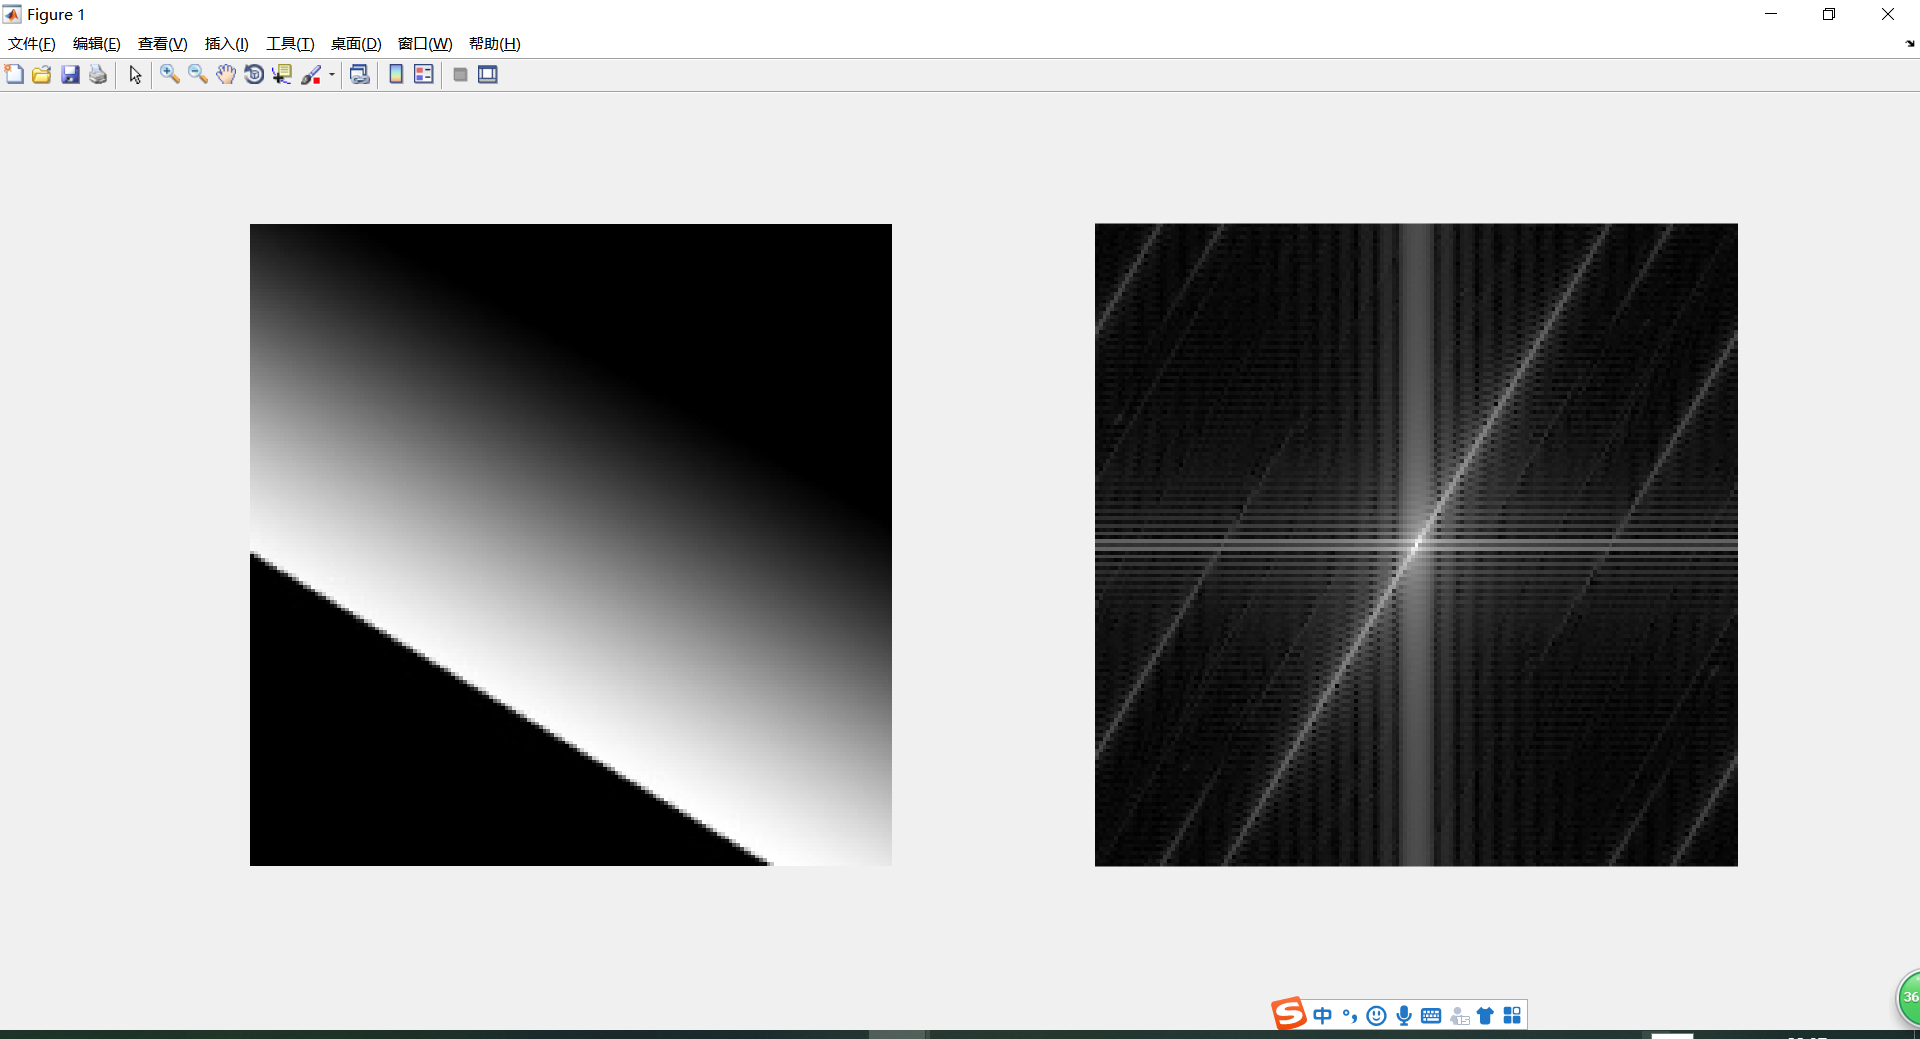
\includegraphics[scale=0.4]{result.png} 
%            	\caption{实验结果} 
%            	\label{result}
%            \end{figure}

            


	\section{总结}
		\indent 本次报告分为两部分:第一部分总结了$RGB$空间和$HSI$空间下的图像增强方法的特点,并通过相应的实验来说明;第二部分总结了几类水下图像增强的方法,并着重介绍了在该领域起着重要作用的暗通道先验算法并对该算法进行了一定程度的复现。
        
        \indent 这次报告的绝大多数时间都花在了暗通道先验算法上。由于这篇论文还有很多地方暂时没有想明白,因此对算法的复现也很难说是成功。从论文里的结果来看,就算没有加$Soft\ Matting$,去雾结果的颜色也不应该有如图\ref{dehaze02}和图\ref{dehaze04}这样大的失真,也不应该有像图\ref{dehaze00}这样多的彩色噪声。暂时还不清楚问题具体出在哪里,只能推测应该是$t$和$A$的求解可能有问题。
        
%			\begin{figure}[H]
%				\centering 
%				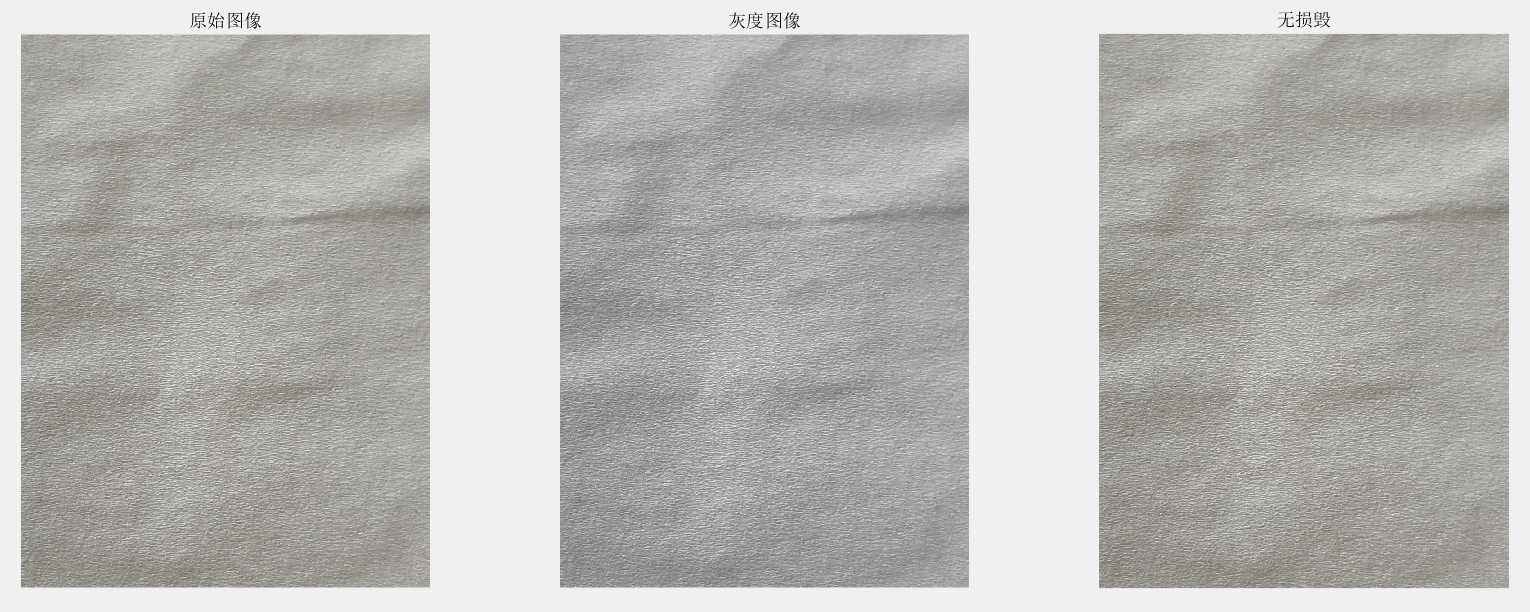
\includegraphics[scale=0.4]{res4.png} 
%				\caption{结果4} 
%				\label{res4}
%			\end{figure}
		

		
%			\begin{figure}[H]
%				\centering 
%				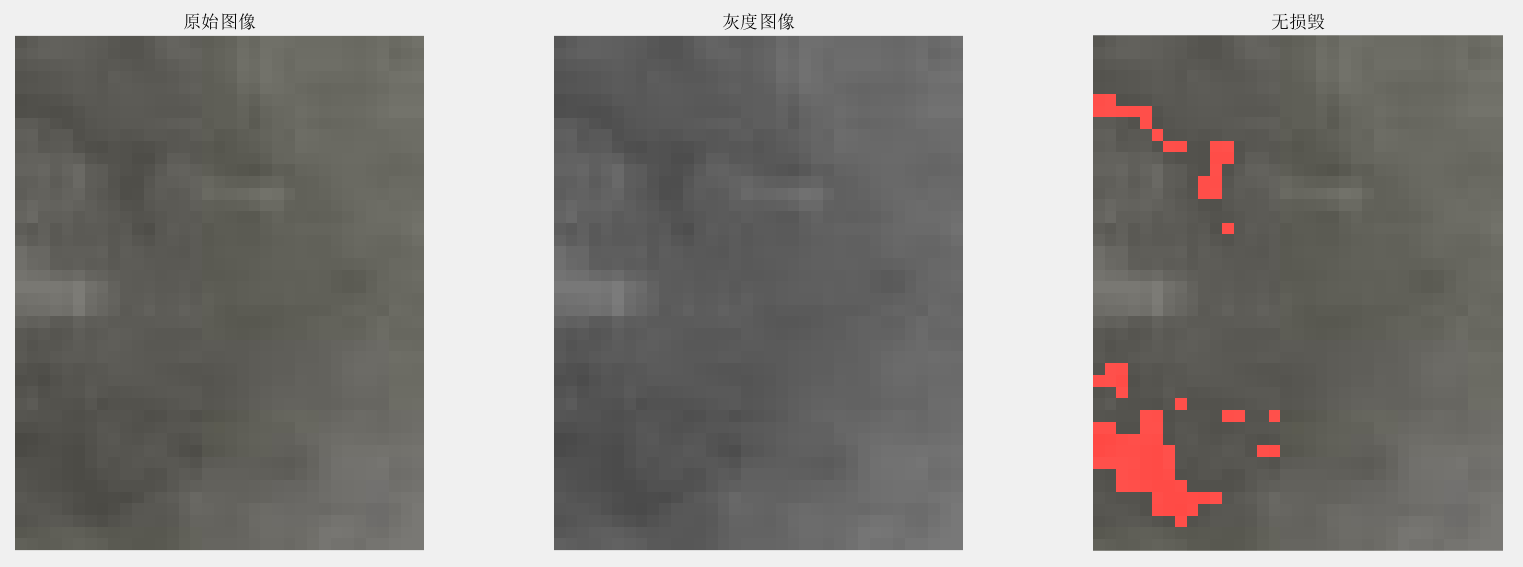
\includegraphics[scale=0.4]{res6.png} 
%				\caption{结果6(截取自结果5的阴影部分)} 
%				\label{res6}
%			\end{figure}
	
	
% 中文文献多个作者用中文逗号“,”连接
%\bibliography{ref.bib}
%\bibliographystyle{abbrv}
\bibliography{ref.bib}


\end{document}